% 04_tcad.tex -- Part 4: device simulation, what calibration can and cannot show. Sources: research_monograph/chapters/
% 14_model_v2_rev.tex (V2 laws, anchors, T2 failure, held-out T3 test), 09_mechanisms_rev.tex (threshold budget, swing
% windows, one-at-a-time leverages, identifiability, contacts), 11_validation_rev.tex (calibration vs validation status),
% M07_provenance.tex (normalised-window swing), M08_c10_campaign.tex (campaign C10 design, stages, S0/S1 results seen
% before register revision 2, budget), M12_multiscale.tex (chain, 2.0 to 6.3 nm arithmetic, one offset vs three films),
% 13_dft_rev.tex (V1 law fitted to published slab DFT), M09_masses_parameters.tex (bulk anchors);
% appendices/MG_corrections.tex (X5, T3); research_record/03_CLAIMS_LEDGER.yaml (C008, C010, C013-C016, C018, C019);
% evidence/FACT_REGISTRY.tsv (FACT-101..103); evidence/derived/multiscale_budget.json. Figures 04_*.pdf:
% tools/fig_04_tcad.py (ATLAS runs 0001-0004, 0014, 0038, 0040, 0060 and data/experimental_clean.csv).
% Blind rules: no ATLAS result from stage S2 on; S0/S1 only as "seen before revision 2" (M08 tab:mono-c10-s1).
\providecommand{\fourTop}{\vspace{-2.5mm}}
\providecommand{\fourC}[1]{{\tiny\color{inkgrey}\,#1}}
\providecommand{\fourAum}{\si{A/\micro\metre}}
\providecommand{\fourNc}{N_{\mathrm{c}}}
\providecommand{\fourEqSkip}{\setlength{\abovedisplayskip}{2pt}\setlength{\belowdisplayskip}{2pt}%
  \setlength{\abovedisplayshortskip}{1pt}\setlength{\belowdisplayshortskip}{2pt}}
\providecommand{\fourAtlas}{\footnote[frame]{Silvaco, \citetitle{AtlasManual}}}
\providecommand{\fourData}{Data: Prof.\ M.-H.\ Lee's group, NTU}
% evidence label at the size of the surrounding \src text (the theme's \lab is \scriptsize)
\providecommand{\fourSrcLab}[1]{{\color{inkgrey}[\textsc{\MakeLowercase{#1}}]}}
% two works, each with its page, in one slide footnote
\providecommand{\fourTwoRefs}[4]{\footnote[frame]{\refcite[#1]{#2}; \refcite[#3]{#4}}}

\partslide{Part 4}{Device simulation: what calibration can and cannot show}

% ---------------------------------------------------------------------------------------------------------------------
\begin{frame}[t]{Confinement enters the model only through material laws}
  \fourTop
  \begin{columns}[T,onlytextwidth]
    \begin{column}{0.54\textwidth}
      {\small\fourEqSkip Silvaco ATLAS\fourAtlas: 2-D drift--diffusion, electrons only, 300\,K, Fermi--Dirac statistics,
        ideal Ohmic contacts.
      \begin{gather*}
        \nabla\!\cdot(\varepsilon\nabla\psi) = q\,\big(n + n_\mathrm{T} - N_{D,\mathrm{eff}}\big), \qquad
        \mathbf{J}_n = \mu\, n\,\nabla E_{Fn}\\
        n = \fourNc\,\mathcal{F}_{1/2}\!\big[(E_{Fn}-\Ec)/\kT\big], \qquad n_\mathrm{T} = \!\int\! g_\mathrm{A} f\,dE\\
        g_\mathrm{A}(E) = \frac{N_t}{W_\mathrm{TA}}\,e^{(E-\Ec)/W_\mathrm{TA}} + g_\mathrm{deep}(E)
      \end{gather*}\par}
      {\footnotesize where $E_{Fn}$ is the electron quasi-Fermi level, $\mathcal{F}_{1/2}$ the Fermi--Dirac integral,
        $f$ the Fermi function, $n_\mathrm{T}$ the trapped electron density and $g_\mathrm{A}$ the acceptor-like trap
        DOS: an exponential tail ($N_t$ states per cm$^3$, width $W_\mathrm{TA}$) plus a deep Gaussian
        $g_\mathrm{deep}$.\par}
    \end{column}
    \begin{column}{0.42\textwidth}
      {\small\fourEqSkip\textbf{Thickness laws} ($t$ in nm)
      \begin{gather*}
        \chi = 4.3\,\mathrm{eV} - \dEc(t), \quad \Eg = 3.05\,\mathrm{eV} + \dEg(t)\\
        \fourNc \propto \big[0.208\,\mzero + \Delta m^{*}(t)\big]^{3/2}\\
        N_t = 2\times10^{19}\,(2/t)^{0.75}\,\mathrm{cm^{-3}}\\
        N_{D,\mathrm{eff}} = 2.5\times10^{17}\,\big[1 + (t/20)^{4}\big]\,\mathrm{cm^{-3}}
      \end{gather*}\par}
      \src{Bulk anchors: 4.3\,eV and 3.05\,eV; 0.208\,$\mzero$\fourTwoRefs{}{Fan2021}{p.~225102-12}{Stokey2021}. The
        first-principles laws supply only the increments. $N_t$ exponent from the paper's trap-density
        ratio\sref[p.~7]{Januar2026}. $N_t$ and $N_{D,\mathrm{eff}}$ laws: V1 and V2; C10 uses $N_t = N_s/t$ and fixed
        donors.}
    \end{column}
  \end{columns}
  \takeaway{No Schr\"odinger solution: confinement acts only via $\chi$, $\Eg$, $\fourNc$ (in C10 also $\mu$, via
    $m^{*}$).}
\end{frame}

% ---------------------------------------------------------------------------------------------------------------------
\begin{frame}[t]{Each device input is either fitted or assumed}
  \fourTop
  {\footnotesize
  \setlength{\tabcolsep}{4pt}
  \renewcommand{\arraystretch}{1.04}
  \begin{tabularx}{\textwidth}{@{}>{\raggedright\arraybackslash}p{6.6cm}>{\raggedright\arraybackslash}X l@{}}
    \toprule
    Input & What it does & Status \\
    \midrule
    $Q_f$ (front sheet): shared; own value at 6.3\,nm in the tuned fit & rigid $\Vg$ shift & \lab{fitted} \\
    $\mu_\mathrm{band}$: one value per film (V1, V2); shared law in C10 & current scale,
      $\times(1-0.287\,\mathrm{nm}/t)^2$ & \lab{fitted} \\
    $N_t$ anchor; tail width $W_\mathrm{TA} = 40$\,meV & swing and turn-on delay\fourC{C015} & \lab{fitted} \\
    $N_{D,\mathrm{eff}}$, compensated & $\le 0.07$\,V of $\Vthcc$\fourC{C016} & \lab{fitted} \\
    $\mathrm{WF}-\chi_\mathrm{bulk} = 0.40$\,eV & rigid offset & \lab{assumed} \\
    Interface traps $D_\mathrm{it}$; deep Gaussian & 0.012\,V; $\le 0.003$\,V of $\Vthcc$ & \lab{assumed} \\
    Confinement law, V1 & fitted to published slab DFT (below) & \lab{assumed} \\
    Confinement laws, V2 and C10 & fitted to this work's DFT points & \lab{fitted} \\
    $\fourNc$ convention (C10, 2.0\,nm: quasi-2-D $N_\mathrm{2D}/t$) & 3-D; C10, 2.0\,nm:
      $1.373\times10^{19}$\cmcu & \lab{assumed} \\
    \bottomrule
  \end{tabularx}\par}
  \src{V1 values unless stated. $\Vthcc$ shares from a 1-D surrogate within 3\,mV of ATLAS. Fitted in V1: the shared
    $Q_f$, the 6.3\,nm $Q_f$, three band mobilities, the tail anchor and width, the donor-law constants. Roughness factor
    $(1-0.287\,\mathrm{nm}/t)^2$ with the roughness length of the device paper\sref[p.~8]{Januar2026}; V1 confinement law fitted to the slab DFT of
    Lin et al.\ and Si et al.\fourTwoRefs{p.~21542}{Lin2022}{p.~504}{Si2021}}
  \takeaway{One film's offset absorbs any confinement law; only shared parameters can be tested.}
\end{frame}

% ---------------------------------------------------------------------------------------------------------------------
\begin{frame}[t]{Calibration matches the anchor films by construction}
  \fourTop
  \begin{columns}[T,onlytextwidth]
    \begin{column}{0.50\textwidth}
      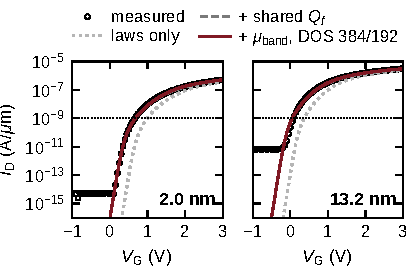
\includegraphics[width=\linewidth]{04_calibration}
      \src{V1 chain at drain bias 0.7\,V: laws only (runs 0001, 0002); + shared $Q_f$ (0003, 0004); final (0038,
        0040: tail-DOS quadrature 384/192, physical deck, band mobility scaled exactly to the measured on-current).
        \fourData\sref{Januar2026}.}
    \end{column}
    \begin{column}{0.47\textwidth}
      {\scriptsize
      \setlength{\tabcolsep}{3pt}
      \renewcommand{\arraystretch}{1.1}
      \begin{tabular}{@{}lcc@{}}
        \toprule
        2.0 / 13.2\,nm & V1 & V2 \\
        \midrule
        Shared $Q_f$ ($10^{12}$\cmsq) & 1.73 & 1.38 \\
        $\mu_\mathrm{band}$ (\cmVs) & 17.69 / 61.60 & 17.54 / 63.21 \\
        $\Delta\Vthcc$ vs measured (mV) & $+19$ / $-29$ & $+6$ / $+21$ \\
        Active RMSE (dec) & 0.043 / 0.081 & 0.065 / 0.097 \\
        \bottomrule
      \end{tabular}\par}
      \src{V1: confinement law fitted to published slab DFT; V2: laws fitted to this work's DFT. On-current exact in
        both; measured $\Vthcc$ 0.662 / 0.083\,V. All rows \fourSrcLab{fitted} (C013).}
      \begin{itemize}\footnotesize
        \item $Q_f$ shifts the curve rigidly (verified to 1\,mV) and $\Id \propto \mu_\mathrm{band}$: one shared
          $Q_f$ sets the threshold pair, $\mu_\mathrm{band}$ each on-current \lab{computed}
        \item 6.3\,nm needs its own $Q_f = 8.7\times10^{10}$\cmsq{} and its own $\mu_\mathrm{band}$ \lab{fitted};
          even then its late, steep turn-on is not reproduced \lab{computed}
      \end{itemize}
    \end{column}
  \end{columns}
  \takeaway{Agreement at the anchors is a calibration, not a test of the thickness laws.}
\end{frame}

% ---------------------------------------------------------------------------------------------------------------------
\begin{frame}[t]{The shared tail fits the deep swing, not every window}
  \fourTop
  {\footnotesize
  \setlength{\tabcolsep}{4pt}
  \renewcommand{\arraystretch}{1.05}
  \begin{tabular*}{\textwidth}{@{}l@{\extracolsep{\fill}}cccl@{}}
    \toprule
    Window & 2.0\,nm & 6.3\,nm & 13.2\,nm & \\
    \midrule
    $10^{-11}$--$10^{-10}$\,\fourAum, meas.\ / sim. & 121.2 / 123.5 & 124.5 / 124.5 & 91.8$^{\ast}$ / 90.9 &
      \lab{fitted} \\
    $(2.15$--$21.5)\times10^{-5}\,I_\mathrm{on}$, meas.\ / sim. & $123.6\pm1.0$ / 126.4 & $122.7\pm9.3$ / 121.3 &
      $115.3\pm2.4$ / 131.3 & \lab{computed}\fourC{C008} \\
    $10^{-10}$--$10^{-9}$\,\fourAum, sim.\ $-$ meas. & $+20$ & $+6$ & $+25$ & \lab{computed} \\
    \bottomrule
  \end{tabular*}\par}
  \src{Swing in mV/dec. V1 calibrated model; the 6.3\,nm curve with its own $Q_f$ and band mobility. $^{\ast}$After
    subtracting the off-state floor (two points); raw 136.1\,mV/dec. Middle row: the normalised window (amendment A1 of
    the extraction protocol). \fourData\sref{Januar2026}.}
  \begin{itemize}\small
    \item One shared $W_\mathrm{TA} = 40$\,meV matches the deepest window within 2.3\,mV/dec at 2.0 and 6.3\,nm
      \lab{fitted}; at 13.2\,nm only after floor subtraction, so it is not claimed there
    \item In the normalised window the 13.2\,nm simulation is $16\pm3$\,mV/dec too high: reported as a finding, not
      tuned away \lab{computed}\fourC{C010}
    \item Above $10^{-10}$\,\fourAum{} the model is too soft in every film: tail filling holds, the V1 tail shape
      does not \lab{inferred}
  \end{itemize}
  \takeaway{Tail filling sets the swing in all films; the V1 tail shape is too soft above $10^{-10}$\,\fourAum.}
\end{frame}

% ---------------------------------------------------------------------------------------------------------------------
\begin{frame}[t]{Every out-of-sample 6.3\,nm threshold prediction failed}
  \fourTop
  \begin{columns}[T,onlytextwidth]
    \begin{column}{0.50\textwidth}
      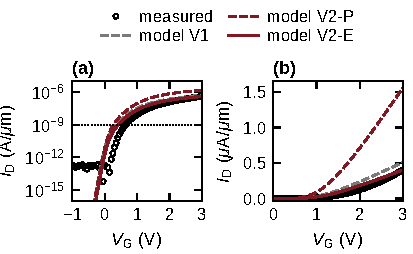
\includegraphics[width=\linewidth]{04_holdout}
      \src{6.3\,nm threshold held out (no $Q_f$ fitted to it). V1 (run 0014) uses the band mobility of the V0 fit of
        this curve, 12.4\cmVs: threshold-only test. V2 (run 0060): P from the registered rule $\propto t^{0.675}$,
        38.39\cmVs; E scaled by 0.2579 to the measured on-current. \fourData\sref{Januar2026}.}
    \end{column}
    \begin{column}{0.47\textwidth}
      \vspace{-1mm}
      {\scriptsize
      \setlength{\tabcolsep}{4pt}
      \renewcommand{\arraystretch}{1.05}
      \begin{tabular}{@{}lcc@{}}
        \toprule
        Prediction (run) & $\Vthcc$ (V) & Miss (V) \\
        \midrule
        V1, shared laws (0014) & 0.350 & \textbf{\textminus0.29} \\
        V2-P, predicted $\mu$ (0060) & 0.270 & \textbf{\textminus0.37} \\
        V2-E, $\mu$ scaled to $I_\mathrm{on}$ (0060) & 0.417 & \textbf{\textminus0.23} \\
        \bottomrule
      \end{tabular}\par}
      \src{Measured 0.644\,V; pass required $|\Delta\Vthcc| \le 0.10$\,V: all three \fourSrcLab{falsified} (C014). V2 registered in commit
        7b75ee6, on-state correction a914165 before the result. The registered T2 anchor check failed at 2.0\,nm (RMSE,
        by 0.001\,dec).}
      \begin{itemize}\footnotesize\setlength{\itemsep}{1pt}
        \item ATLAS matched the registered T3 thresholds within 0.3\,mV \lab{computed}
        \item DFT laws shrink the miss by only about 0.04\,V; the linear threshold is 0.58\,V too low; rule P gives
          four times $I_\mathrm{on}$ \lab{computed}
        \item The computed $\dEc$ law, applied rigidly, gives $-0.21$ to $-0.22$\,V from 2.0 to 6.3\,nm; measured
          $-0.018$\,V \lab{derived}
      \end{itemize}
    \end{column}
  \end{columns}
  \takeaway{The model describes the anchor films; it does not predict the thickness dependence.}
\end{frame}

% ---------------------------------------------------------------------------------------------------------------------
\begin{frame}[t]{One transfer curve fixes combinations, not parameters}
  \fourTop
  \begin{columns}[T,onlytextwidth]
    \begin{column}{0.53\textwidth}
      {\scriptsize
      \setlength{\tabcolsep}{4pt}
      \renewcommand{\arraystretch}{1.2}
      \begin{tabular}{@{}lrrl@{}}
        \toprule
        Change at 2.0\,nm & $\Delta\Vthcc$ (V) & $\Delta$SS (mV/dec) & Action \\
        \midrule
        Gate WF $+0.1$\,eV & $+0.100$ & 0 & rigid \\
        $\chi$ $-0.1$ / $+0.1$\,eV & $+0.100$ / $-0.100$ & 0 & rigid \\
        Confinement off & $-0.316$ & $+15.3$ & near-rigid \\
        $N_t\times1.5$ & $+0.082$ & $+49.0$ & slope, delay \\
        $m^{*}\times1.3$ (via $\fourNc$) & $-0.044$ & $-18.0$ & slope \\
        $W_\mathrm{TA}$ $+5$\,meV & $+0.020$ & $+4.6$ & slope \\
        $D_\mathrm{it}\times3$ & $+0.025$ & -- & small shift \\
        $N_D\times2$ & $-0.009$ & -- & negligible \\
        $\varepsilon_\mathrm{IWO} = 10.55$ & $-0.001$ & -- & negligible \\
        \bottomrule
      \end{tabular}\par}
      \src{One-at-a-time ATLAS pairs \fourSrcLab{computed} (runs 0048, 0020/0021, 0016, 0023, 0050, 0024, 0025, 0022,
        0026); SS over $10^{-10}$--$10^{-9}$\,A/\textmu m. On-current change: $-25.1$\,\% for $N_t\times1.5$,
        $+21.4$\,\% for confinement off. No Jacobian or profile analysis was made.}
    \end{column}
    \begin{column}{0.44\textwidth}
      \begin{itemize}\footnotesize
        \item Work function, affinity, uniform fixed charge and confinement shift act as one number per film:
          $\dEc(2\,\mathrm{nm}) = 0.353$\,eV $\equiv 1.97\times10^{12}$\cmsq{} of fixed charge
          \lab{computed}\fourC{C018}
        \item $\mu_\mathrm{band}$ trades with $N_t$: on $I_\mathrm{on}$, $N_t\times1.5 \equiv \mu\times1.33$; series
          resistance trades with the tail exponent \lab{derived}\fourC{C018}
        \item One shared offset fits the three thresholds equally well with and without confinement: rms 0.136 vs
          0.133\,V \lab{computed}
        \item Separating them needs C--V flat band against $t$, the optical gap, gated Hall and a transfer-length
          series
      \end{itemize}
    \end{column}
  \end{columns}
  \takeaway{The calibrated set is one member of a family of equivalent calibrations, not an extraction.}
\end{frame}

% ---------------------------------------------------------------------------------------------------------------------
\begin{frame}[t]{Thickness-independent contacts cannot create the trend}
  \fourTop
  \begin{columns}[T,onlytextwidth]
    \begin{column}{0.38\textwidth}
      \centering
      \vspace{2mm}
      \begin{tikzpicture}[x=0.80mm,y=1.2mm,line width=0.5pt,font=\footnotesize]
        % circuit: source - R_S - channel - R_D - drain
        \draw (0,10) -- (6,10);
        \draw (6,8) rectangle (14,12); \node[above] at (10,12) {$R_\mathrm{S}$};
        \draw (14,10) -- (19,10);
        \draw[ntumaroon] (19,7.5) rectangle (35,12.5); \node at (27,10) {$R_\mathrm{ch}(\Vg)$};
        \draw (35,10) -- (40,10);
        \draw (40,8) rectangle (48,12); \node[above] at (44,12) {$R_\mathrm{D}$};
        \draw (48,10) -- (54,10);
        \fill (0,10) circle[radius=0.7mm]; \fill (54,10) circle[radius=0.7mm];
        \node[left] at (-0.5,10) {S}; \node[right] at (54.5,10) {D};
        \draw[{Latex[length=1.5mm]}-{Latex[length=1.5mm]}] (0,19) -- (54,19);
        \node[fill=white,inner sep=1pt] at (27,19) {$\Vd = 0.7$\,V};
        % voltage share required at 2.0 nm (hypothetical)
        \fill[black!25] (0,0) rectangle (22.4,3.5);
        \fill[black!25] (31.6,0) rectangle (54,3.5);
        \draw (0,0) rectangle (54,3.5);
        \draw (22.4,0) -- (22.4,3.5); \draw (31.6,0) -- (31.6,3.5);
        \node[below,align=center,text width=44mm,font=\scriptsize] at (27,-0.8) {required at 2.0\,nm: 83\,\% of
          $\Vd$ across the contacts (grey), 17\,\% across the channel};
      \end{tikzpicture}
      \src{Schematic; the split is the hypothetical needed for contacts alone to cause the 2.0\,nm deficit.}
    \end{column}
    \begin{column}{0.59\textwidth}
      \begin{itemize}\footnotesize
        \item Contacts alone would need $R_\mathrm{sd}W \approx 1.15\times10^{6}\,\Omega\,\si{\micro\metre}$ at
          2.0\,nm: $\rho_c \approx 0.26\,\Omega\,\mathrm{cm^2}$, $L_T \approx 45\,\si{\micro\metre}$ \lab{derived}
        \item That drops 83\,\% of $\Vd$ in the contacts; per contact (about 570\,$\Omega$\,mm) it is about 5700
          times the contact resistance of related metal/\InO{} contacts, below 0.1\,$\Omega$\,mm\sref[p.~167]{Si2022}
        \item Wrong sign: $\theta_\mathrm{net} = -0.10$ / $-0.12$ / $-0.046$\,V$^{-1}$ (2.0 / 6.3 / 13.2\,nm);
          series resistance needs the opposite sign \lab{derived}
        \item Wrong direction: at fixed $\rho_c$ the contact share scales as $R_\mathrm{sh}^{-1/2}$, so a common
          contact penalises the thick film \lab{derived}\fourC{C019}
        \item Inside the calibrated trap model: $R_\mathrm{sd}W \lesssim 5\times10^{4}\,\Omega\,\si{\micro\metre}$
          ($\le 4$\,\%) at 2.0\,nm, $\lesssim$ 1--2$\times10^{4}\,\Omega\,\si{\micro\metre}$ (4--9\,\%) at
          13.2\,nm \lab{fitted}
      \end{itemize}
    \end{column}
  \end{columns}
  \takeaway{Contacts do not make the trend; a minor share needs a transfer-length series to settle.}
\end{frame}

% ---------------------------------------------------------------------------------------------------------------------
\begin{frame}[t]{Campaign C10 tests one parameter set shared by all three films}
  \fourTop
  \begin{columns}[T,onlytextwidth]
    \begin{column}{0.50\textwidth}
      \begin{itemize}\footnotesize
        \item Five shared fitted parameters: offset $\Delta V_0$ (via $Q_f$), $\mu_\infty$, length $\ell$, tail sheet
          $N_s$ ($N_t = N_s/t$), $W_\mathrm{TA}$; no per-film charge or mobility; DFT laws in $\chi$, $\Eg$, $\fourNc$,
          $\mu$
      \end{itemize}
      {\footnotesize\fourEqSkip
      \[ \mu_\mathrm{band}(t) = \mu_\infty\,\frac{0.208\,\mzero}{m^{*}(t)}\,\frac{1}{1+\ell/t}
         \Big(1-\frac{0.287\,\mathrm{nm}}{t}\Big)^{2} \]
      where $m^{*}(t) = 0.208\,\mzero + \Delta m^{*}(t)$ (DFT increment) and the last factor is the existing roughness
      term.\par}
      \begin{itemize}\footnotesize
        \item The mass ratio gives only $\times0.83$ from 13.2 to 2.0\,nm, about 14\,\% of the logarithmic drop the
          calibrated models need \lab{derived}; by design $\ell$ carries the rest (H-D, sealed)
        \item $\Delta V_0$, $\mu_\infty$, $\ell$ are profiled offline by exact transformations; three degrees of
          freedom remain
        \item Acceptance, stop rules and the expected 6.3\,nm failure were fixed before any launch
      \end{itemize}
    \end{column}
    \begin{column}{0.47\textwidth}
      {\scriptsize
      \setlength{\tabcolsep}{3pt}
      \renewcommand{\arraystretch}{1.08}
      \begin{tabularx}{\linewidth}{@{}l r>{\raggedright\arraybackslash}X@{}}
        \toprule
        Stage & Launches & Content \\
        \midrule
        S0 smoke & 2 & 2.0\,nm baseline; gate tunnelling \\
        S1 baselines & 7 & baselines; numerics; 3-D $\fourNc$ \\
        \midrule
        S2 off-state floor & 17 & generation; leakage; ungated strip \\
        S3 model form & 27 & confinement off; branches \\
        S4 calibration & 69 & space-filling and adaptive \\
        S5 leave-one-out & 30 & held-out film never tuned \\
        S6 sensitivity & 27 & DFT low/high; mass; $N_D$; traps \\
        S7 31.8\,nm & 2 & frozen model, never fitted \\
        \midrule
        Reserve & 19 & total 200 \\
        \bottomrule
      \end{tabularx}\par}
      \src{Planned launches, approved 10 Oct 2026 (D-13); regenerated matrix: 184 + 16 reserve (recorded
        inconsistency). S0/S1 used 14 launches (S0-02 needed six), seen before the register freeze; 17 of 200 used by
        14 Oct.}
    \end{column}
  \end{columns}
  \takeaway{With one offset for all three films, the first-principles inputs can fail for the first time.}
\end{frame}

% ---------------------------------------------------------------------------------------------------------------------
\begin{frame}[t]{The $\fourNc$ convention alone moves the 2.0\,nm threshold by 142\,mV}
  \fourTop
  \begin{columns}[T,onlytextwidth]
    \begin{column}{0.57\textwidth}
      {\scriptsize
      \setlength{\tabcolsep}{3pt}
      \renewcommand{\arraystretch}{1.05}
      \begin{tabularx}{\linewidth}{@{}l>{\raggedright\arraybackslash}p{3.05cm}>{\raggedright\arraybackslash}X@{}}
        \toprule
        Run & Test & Result \\
        \midrule
        S1-01 & 6.3\,nm baseline & RMSE 1.18\,dec; $\Id(3\,\mathrm{V})$ $\times4.87$ \\
        S1-02 & 13.2\,nm baseline & RMSE 0.056\,dec \\
        S1-03 & 13.2\,nm, mesh $\times0.7$ & pass, $\Delta$RMSE $-0.0005$\,dec \\
        S1-04 & 2.0\,nm, DOS quadrature $\times2$ & pass, $\Delta$RMSE $-0.00002$\,dec \\
        S1-05 & 2.0\,nm, 3-D instead of quasi-2-D $\fourNc$ & $\Delta\Vthcc$ $+142$\,mV vs registered $+40$ to
          $+70$\,mV: \textbf{failed}; $\Delta$SS $+49$\,mV/dec; RMSE $0.367\to0.053$\,dec \\
        \bottomrule
      \end{tabularx}\par}
      \src{Stage S1 (runs 0061--0074 with S0), seen before register revision 2; model-internal, at the shared start
        parameters \fourSrcLab{computed}. $\Id(3\,\mathrm{V})$ relative to the measured value. S1-06 (13.2\,nm, two carriers) timed out: unresolved. S1-07 (ATLAS check of the
        offline profiling) passed, $\le 2.05\times10^{-4}$\,dec.}
      \begin{itemize}\footnotesize
        \item Quasi-2-D $\fourNc$ at 2.0\,nm: within 0.86\,mV of true 2-D statistics at threshold, $I_\mathrm{on}$
          about 7--8\,\% high \lab{inferred}
        \item $\fourNc$ is degenerate with $Q_f$ and trap densities: each fitted value must name its convention
          \lab{inferred}
      \end{itemize}
    \end{column}
    \begin{column}{0.40\textwidth}
      \centering
      \begin{tikzpicture}[x=0.32mm,y=1mm,font=\scriptsize]
        \fill[black!15] (40,0) rectangle (70,4);
        \draw[line width=0.5pt] (0,0) -- (160,0);
        \foreach \x in {0,40,80,120,160} {\draw (\x,0) -- (\x,-1.2); \node[below] at (\x,-1.2) {\x};}
        \node[above] at (55,4) {registered $+40$ to $+70$};
        \fill[ntumaroon] (142,2) circle[radius=0.8mm];
        \node[above,text=ntumaroon] at (142,3.5) {S1-05: $+142$};
        \node[below] at (80,-5.5) {$\Delta\Vthcc$ at 2.0\,nm (mV)};
      \end{tikzpicture}
      \src{Registered expectation (register revision 1) and run S1-05.}
      \begin{itemize}\footnotesize
        \item Audit A13: no implementation error; of the $+142$\,mV, $+37.5$\,mV from the statistics and
          $+89.5$\,mV from extra charge in the 40\,meV tail (127\,mV itemised) \lab{computed}
        \item The effective slope factor at $10^{-9}$\,\fourAum{} is about 3.5, not the 1.47 assumed in the
          registration \lab{computed}
      \end{itemize}
    \end{column}
  \end{columns}
  \takeaway{The DOS convention alone moves $\Vthcc$ by a third to two thirds of a 6.3\,nm miss.}
\end{frame}

% ---------------------------------------------------------------------------------------------------------------------
\begin{frame}[t]{Sealed stages S2--S7 decide transfer, not device physics}
  \fourTop
  \begin{center}
    \begin{minipage}{0.86\textwidth}
      \sealed{Outcomes of stages S2--S7 of campaign C10 (every launch after the register freeze of 10 Oct 2026)}
    \end{minipage}
  \end{center}
  \vspace{4mm}
  \begin{columns}[T,onlytextwidth]
    \begin{column}{0.56\textwidth}
      {\scriptsize
      \setlength{\tabcolsep}{3pt}
      \renewcommand{\arraystretch}{1.05}
      \begin{tabularx}{\linewidth}{@{}l>{\raggedright\arraybackslash}X l@{}}
        \toprule
        Stage & Question it will decide & Register \\
        \midrule
        S2 & can gate leakage, generation or an ungated strip give the off-state floors? & H-A, H-B, H-C \\
        S3 & how much threshold the first-principles inputs carry (all off) & H-E \\
        S4 & is a $1/t$ scattering term needed in the band mobility? & H-D \\
        S4, S5 & does one set transfer to each held-out film; what remains at 6.3\,nm? & H-F, H-J \\
        S6, S7 & sensitivity to the inputs; 31.8\,nm with the frozen model, never fitted & -- \\
        \bottomrule
      \end{tabularx}\par}
      \src{Registered predictions: Part 3. Stage-to-hypothesis assignment ours, from the stage contents. Stop rule: if
        after the first calibration sub-stage the best shared fit exceeds 0.30\,dec rms log-current error with
        systematic 6.3\,nm residuals, the shared model is reported as failed, with no per-film rescue.}
    \end{column}
    \begin{column}{0.41\textwidth}
      {\small\textbf{What C10 cannot establish}\par}
      \begin{itemize}\small
        \item The device physics: four single-device curves, one $\Vd$ and no gate current leave several mechanisms
          indistinguishable
        \item Confinement: not identifiable from transfer curves\fourC{C018}
        \item Success on all three films would still be a calibration
      \end{itemize}
    \end{column}
  \end{columns}
  \takeaway{Decisive next step: replicate devices, C--V and the optical gap versus thickness.}
\end{frame}
